\documentclass[floatsintext,man]{apa6}

\usepackage{amssymb,amsmath}
\usepackage{ifxetex,ifluatex}
\usepackage{fixltx2e} % provides \textsubscript
\ifnum 0\ifxetex 1\fi\ifluatex 1\fi=0 % if pdftex
  \usepackage[T1]{fontenc}
  \usepackage[utf8]{inputenc}
\else % if luatex or xelatex
  \ifxetex
    \usepackage{mathspec}
    \usepackage{xltxtra,xunicode}
  \else
    \usepackage{fontspec}
  \fi
  \defaultfontfeatures{Mapping=tex-text,Scale=MatchLowercase}
  \newcommand{\euro}{€}
\fi
% use upquote if available, for straight quotes in verbatim environments
\IfFileExists{upquote.sty}{\usepackage{upquote}}{}
% use microtype if available
\IfFileExists{microtype.sty}{\usepackage{microtype}}{}

% Table formatting
\usepackage{longtable, booktabs}
\usepackage{lscape}
% \usepackage[counterclockwise]{rotating}   % Landscape page setup for large tables
\usepackage{multirow}		% Table styling
\usepackage{tabularx}		% Control Column width
\usepackage[flushleft]{threeparttable}	% Allows for three part tables with a specified notes section
\usepackage{threeparttablex}            % Lets threeparttable work with longtable

% Create new environments so endfloat can handle them
% \newenvironment{ltable}
%   {\begin{landscape}\begin{center}\begin{threeparttable}}
%   {\end{threeparttable}\end{center}\end{landscape}}

\newenvironment{lltable}
  {\begin{landscape}\begin{center}\begin{ThreePartTable}}
  {\end{ThreePartTable}\end{center}\end{landscape}}




% The following enables adjusting longtable caption width to table width
% Solution found at http://golatex.de/longtable-mit-caption-so-breit-wie-die-tabelle-t15767.html
\makeatletter
\newcommand\LastLTentrywidth{1em}
\newlength\longtablewidth
\setlength{\longtablewidth}{1in}
\newcommand\getlongtablewidth{%
 \begingroup
  \ifcsname LT@\roman{LT@tables}\endcsname
  \global\longtablewidth=0pt
  \renewcommand\LT@entry[2]{\global\advance\longtablewidth by ##2\relax\gdef\LastLTentrywidth{##2}}%
  \@nameuse{LT@\roman{LT@tables}}%
  \fi
\endgroup}


  \usepackage{graphicx}
  \makeatletter
  \def\maxwidth{\ifdim\Gin@nat@width>\linewidth\linewidth\else\Gin@nat@width\fi}
  \def\maxheight{\ifdim\Gin@nat@height>\textheight\textheight\else\Gin@nat@height\fi}
  \makeatother
  % Scale images if necessary, so that they will not overflow the page
  % margins by default, and it is still possible to overwrite the defaults
  % using explicit options in \includegraphics[width, height, ...]{}
  \setkeys{Gin}{width=\maxwidth,height=\maxheight,keepaspectratio}
\ifxetex
  \usepackage[setpagesize=false, % page size defined by xetex
              unicode=false, % unicode breaks when used with xetex
              xetex]{hyperref}
\else
  \usepackage[unicode=true]{hyperref}
\fi
\hypersetup{breaklinks=true,
            pdfauthor={},
            pdftitle={Learning to Interpret a Disjunction},
            colorlinks=true,
            citecolor=blue,
            urlcolor=blue,
            linkcolor=black,
            pdfborder={0 0 0}}
\urlstyle{same}  % don't use monospace font for urls

\setlength{\parindent}{0pt}
%\setlength{\parskip}{0pt plus 0pt minus 0pt}

\setlength{\emergencystretch}{3em}  % prevent overfull lines


% Manuscript styling
\captionsetup{font=singlespacing,justification=justified}
\usepackage{csquotes}
\usepackage{upgreek}

 % Line numbering
  \usepackage{lineno}
  \linenumbers


\usepackage{tikz} % Variable definition to generate author note

% fix for \tightlist problem in pandoc 1.14
\providecommand{\tightlist}{%
  \setlength{\itemsep}{0pt}\setlength{\parskip}{0pt}}

% Essential manuscript parts
  \title{Learning to Interpret a Disjunction}

  \shorttitle{Learning Disjunction}


  \author{Masoud Jasbi\textsuperscript{1}, Akshay Jaggi\textsuperscript{2}, \& Michael C. Frank\textsuperscript{2}}

  % \def\affdep{{"", "", ""}}%
  % \def\affcity{{"", "", ""}}%

  \affiliation{
    \vspace{0.5cm}
          \textsuperscript{1} Harvard University\\
          \textsuperscript{2} Stanford University  }

  \authornote{
    Add complete departmental affiliations for each author here. Each new
    line herein must be indented, like this line.
    
    Enter author note here.
    
    Correspondence concerning this article should be addressed to Masoud
    Jasbi, Postal address. E-mail:
    \href{mailto:masoud_jasbi@fas.harvard.edu}{\nolinkurl{masoud\_jasbi@fas.harvard.edu}}
  }


  \abstract{Enter abstract here. Each new line herein must be indented, like this
line.}
  \keywords{keywords \\

    \indent Word count: X
  }





\usepackage{amsthm}
\newtheorem{theorem}{Theorem}
\newtheorem{lemma}{Lemma}
\theoremstyle{definition}
\newtheorem{definition}{Definition}
\newtheorem{corollary}{Corollary}
\newtheorem{proposition}{Proposition}
\theoremstyle{definition}
\newtheorem{example}{Example}
\theoremstyle{definition}
\newtheorem{exercise}{Exercise}
\theoremstyle{remark}
\newtheorem*{remark}{Remark}
\newtheorem*{solution}{Solution}
\begin{document}

\maketitle

\setcounter{secnumdepth}{0}



\section{Introduction}\label{introduction}

\section{Study 1: Disjunction in adult
conversations}\label{study-1-disjunction-in-adult-conversations}

\section{Study 2: Disjunction in child-directed
speech}\label{study-2-disjunction-in-child-directed-speech}

\subsection{Methods}\label{methods}

For samples of parents' and children's speech, this study used the
online database \href{childes-db.stanford.edu}{childes-db} and its
associated R programming package \texttt{childesr} (Sanchez et al.,
2018). Childes-db is an online interface to the child language
components of \href{https://talkbank.org/}{TalkBank}, namely
\href{https://childes.talkbank.org/}{CHILDES} (MacWhinney, 2000) and
\href{https://phonbank.talkbank.org/}{PhonBank}. Two collections of
corpora were selected: English-North America and English-UK. All word
tokens were tagged for the following information: 1. The speaker role
(mother, father, child), 2. the age of the child when the word was
produced, 3. the type of the utterance the word appeared in
(declarative, question, imperative, other), and 4. whether the word was
\emph{and}, \emph{or}, or neither.

\begin{figure}[tb]

{\centering 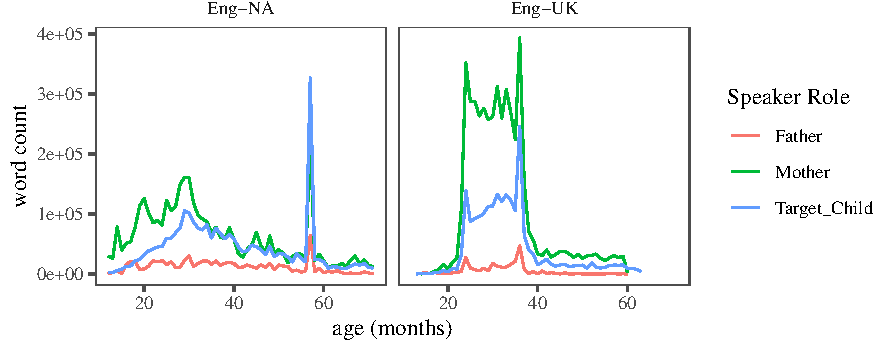
\includegraphics{figs/corpusDensityPlot-1} 

}

\caption{Frequency for all the words in the North America and UK corpora of CHILDES.}\label{fig:corpusDensityPlot}
\end{figure}

\begin{figure}[tb]

{\centering 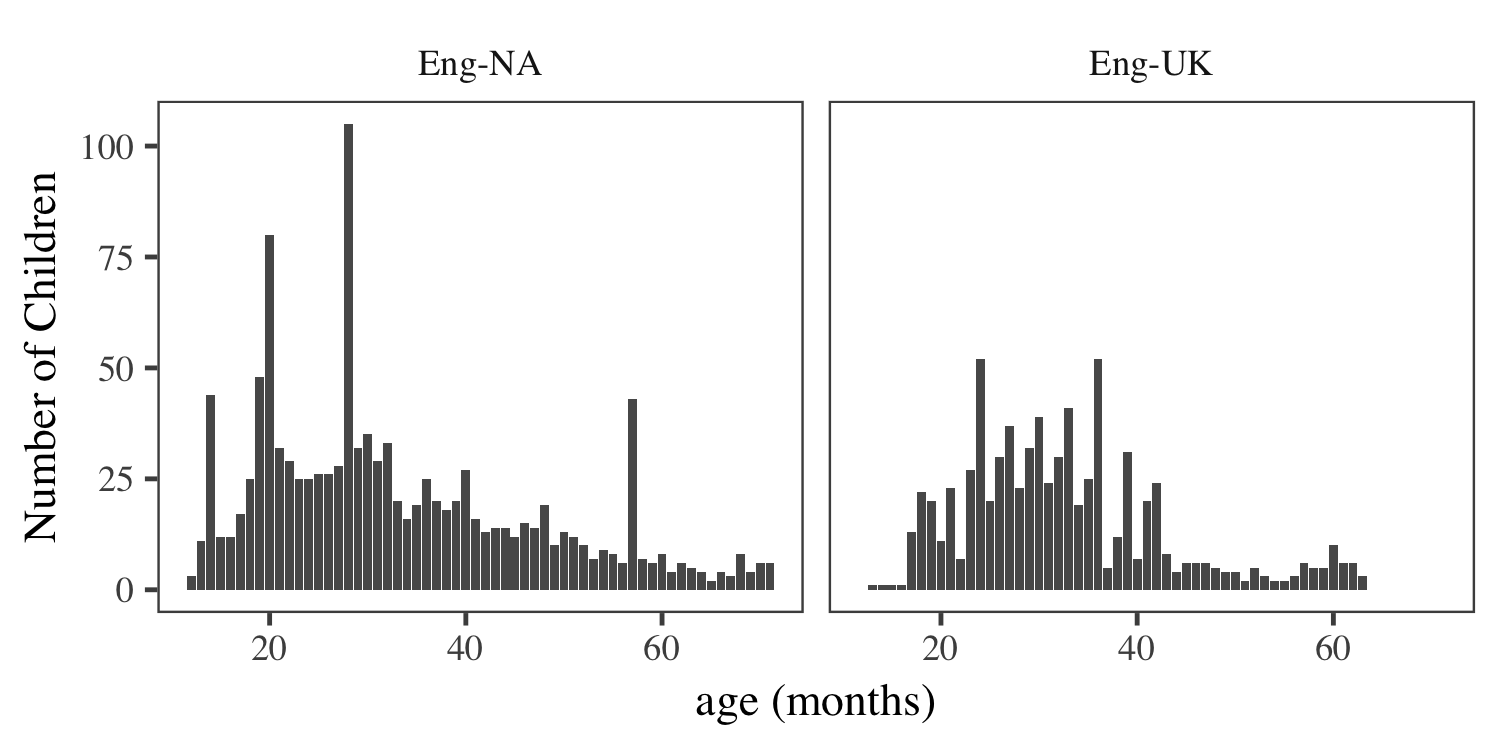
\includegraphics{figs/childDensityPlot-1} 

}

\caption{The number of children represented at different ages in the North America and UK corpora in CHILDES.}\label{fig:childDensityPlot}
\end{figure}

\subsubsection{Exclusion Criteria}\label{exclusion-criteria}

First, observations (tokens) that were coded as unintelligible were
excluded (N = 290,119). Second, observations that had missing
information on children's age were excluded (N = 1,042,478). Third,
observations outside the age range of 1 to 6 years were excluded (N =
686,870). This exclusion was mainly because there was not much data
outside this age range. Figure \ref{fig:ageDistPlot} shows the
distribution of transcripts based on the age of the child at recording
time. The mean age is shown with a red vertical line (Mean Age = 3.73,
SD = 2.21). The collection contained the speech of 504 children and
their parents after the exclusions.

\paragraph{Procedure}\label{procedure}

Each token was marked for the utterance type that the token appeared in.
This study grouped utterance types into four main categories:
\enquote{declarative}, \enquote{question}, \enquote{imperative}, and
\enquote{other}. Utterance type categorization followed the convention
used in the
\href{https://talkbank.org/manuals/CHAT.html\#_Toc486414422}{TalkBank
manual}. The utterance types are similar to sentence types (declarative,
interrogative, imperative) with one exception: the category
\enquote{question} consists of interrogatives as well as rising
declaratives (i.e.~declaratives with rising question intonation). In the
transcripts, declaratives are marked with a period, questions with a
question mark, and imperatives with an exclamation mark. It is important
to note that the manual also provides
\href{https://talkbank.org/manuals/CHAT.html\#_Toc486414431}{terminators
for special-type utterances}. Among the special type utterances, this
study included the following in the category \enquote{questions}:
trailing off of a question, question with exclamation, interruption of a
question, and self-interrupted question. The category imperatives also
included \enquote{emphatic imperatives}. The rest of the special type
utterances such as \enquote{interruptions} and \enquote{trailing off}
were included in the category \enquote{other}.

\begin{figure}
\centering
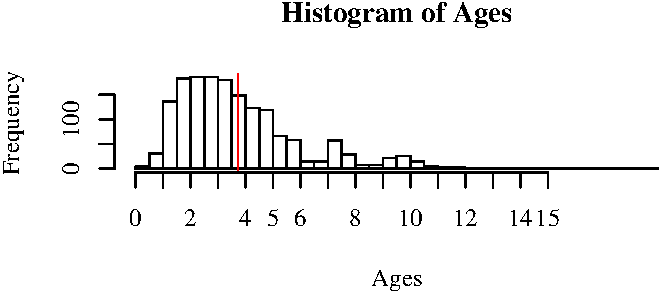
\includegraphics{figs/ageDistPlot-1.pdf}
\caption{\label{fig:ageDistPlot}Distribution of children's ages at recording
times. Mean age is shown using a red vertical line.}
\end{figure}

\subsubsection{Properties of the CHILDES
Corpora}\label{properties-of-the-childes-corpora}

In this section, I report some results on the distribution of words and
utterances among the speakers in our collection of corpora. The
collection contained 14,159,609 words. Table (\ref{tab:countTable})
shows the total number of \emph{and}'s, \emph{or}'s, and words in the
speech of children, fathers, and mothers. The collection contains 8.80
times more words for mothers compared to fathers and 1.80 more words for
mothers compared to children. Therefore, the collection is more
representative of the mother-child interactions than father-child
interactions. Compared to \emph{or}, the word \emph{and} is 10.80 times
more likely in the speech of mothers, 9.20 times more likely in the
speech of fathers, and 30.30 times more likely in the speech of
children. Overall, \emph{and} is 13.35 times more likely than \emph{or}
in this collection which is close to the rate reported by Morris (2008).
He extracted 5,994 instances of \emph{and} and 465 instances of
\emph{or} and found that overall, \emph{and} was 12.89 times more
frequent than \emph{or} in parent-child interactions.

\begin{table}

\caption{\label{tab:countTable}Number of \textit{and}'s, \textit{or}'s, and the total number of words in the speech of children and their parents in English-North America and English-UK collections after exclusions.}
\centering
\begin{tabular}[t]{l|r|r|r}
\hline
Speaker Role & and & or & total\\
\hline
Father & 15,488 & 1,683 & 967,075\\
\hline
Mother & 153,781 & 14,288 & 8,511,478\\
\hline
Target\_Child & 78,443 & 2,590 & 4,681,056\\
\hline
\end{tabular}
\end{table}

Figure \ref{fig:wordsByAge} shows the number of words spoken by parents
and children at each month of the child's development. The words in the
collection are not distributed uniformly and there is a high
concentration of data between the ages of 20 and 40 months (around 2 to
3 years of age). There is also a high concentration around 60 months (5
years of age). The speech of fathers shows a relatively low word-count
across all ages. Therefore, in our analyses we should be more cautious
in drawing conclusions about the speech of fathers generally, and the
speech of mothers and children after age 5.

\begin{figure}[tb]

{\centering 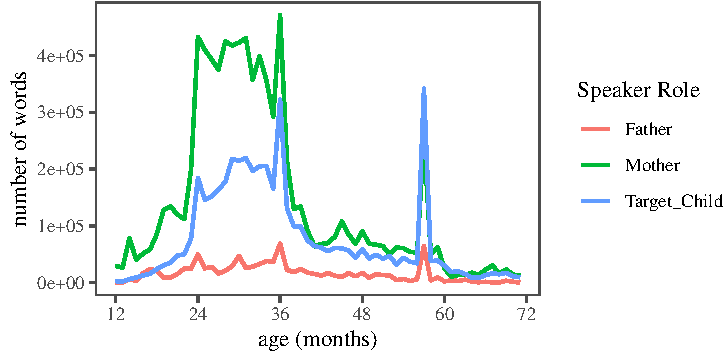
\includegraphics{figs/wordsByAge-1} 

}

\caption{The number of words in the corpora for parents and children in each month of children's development.}\label{fig:wordsByAge}
\end{figure}

The distribution of function words is sensitive to the type of utterance
or more broadly the type of speech act produced by speakers. For
example, it is not surprising to hear a parent say \enquote{go to your
room} but a child saying the same to a parent is unexpected. If a
function word commonly occurs in such speech acts, it is unlikely to be
produced by children, even though they may understand it very well.
Therefore, it is important to check the distribution of speech acts in
corpora when studying different function words. Since it is hard to
classify and quantify speech acts automatically, here I use utterance
type as a proxy for speech acts. I investigate the distribution of
declaratives, questions, and imperatives in this collection of corpora
on parent-child interactions. Figure \ref{fig:totalUtteranceTypePlot}
shows the distribution of different utterance types in the speech of
parents and children. Overall, most utterances are either declaratives
or questions, and there are more declaratives than questions in this
collection. While mothers and fathers show similar proportions of
declaratives and questions in their speech, children produce a lower
proportion of questions and higher proportion of declaratives than their
parents.

\begin{figure}[tb]

{\centering 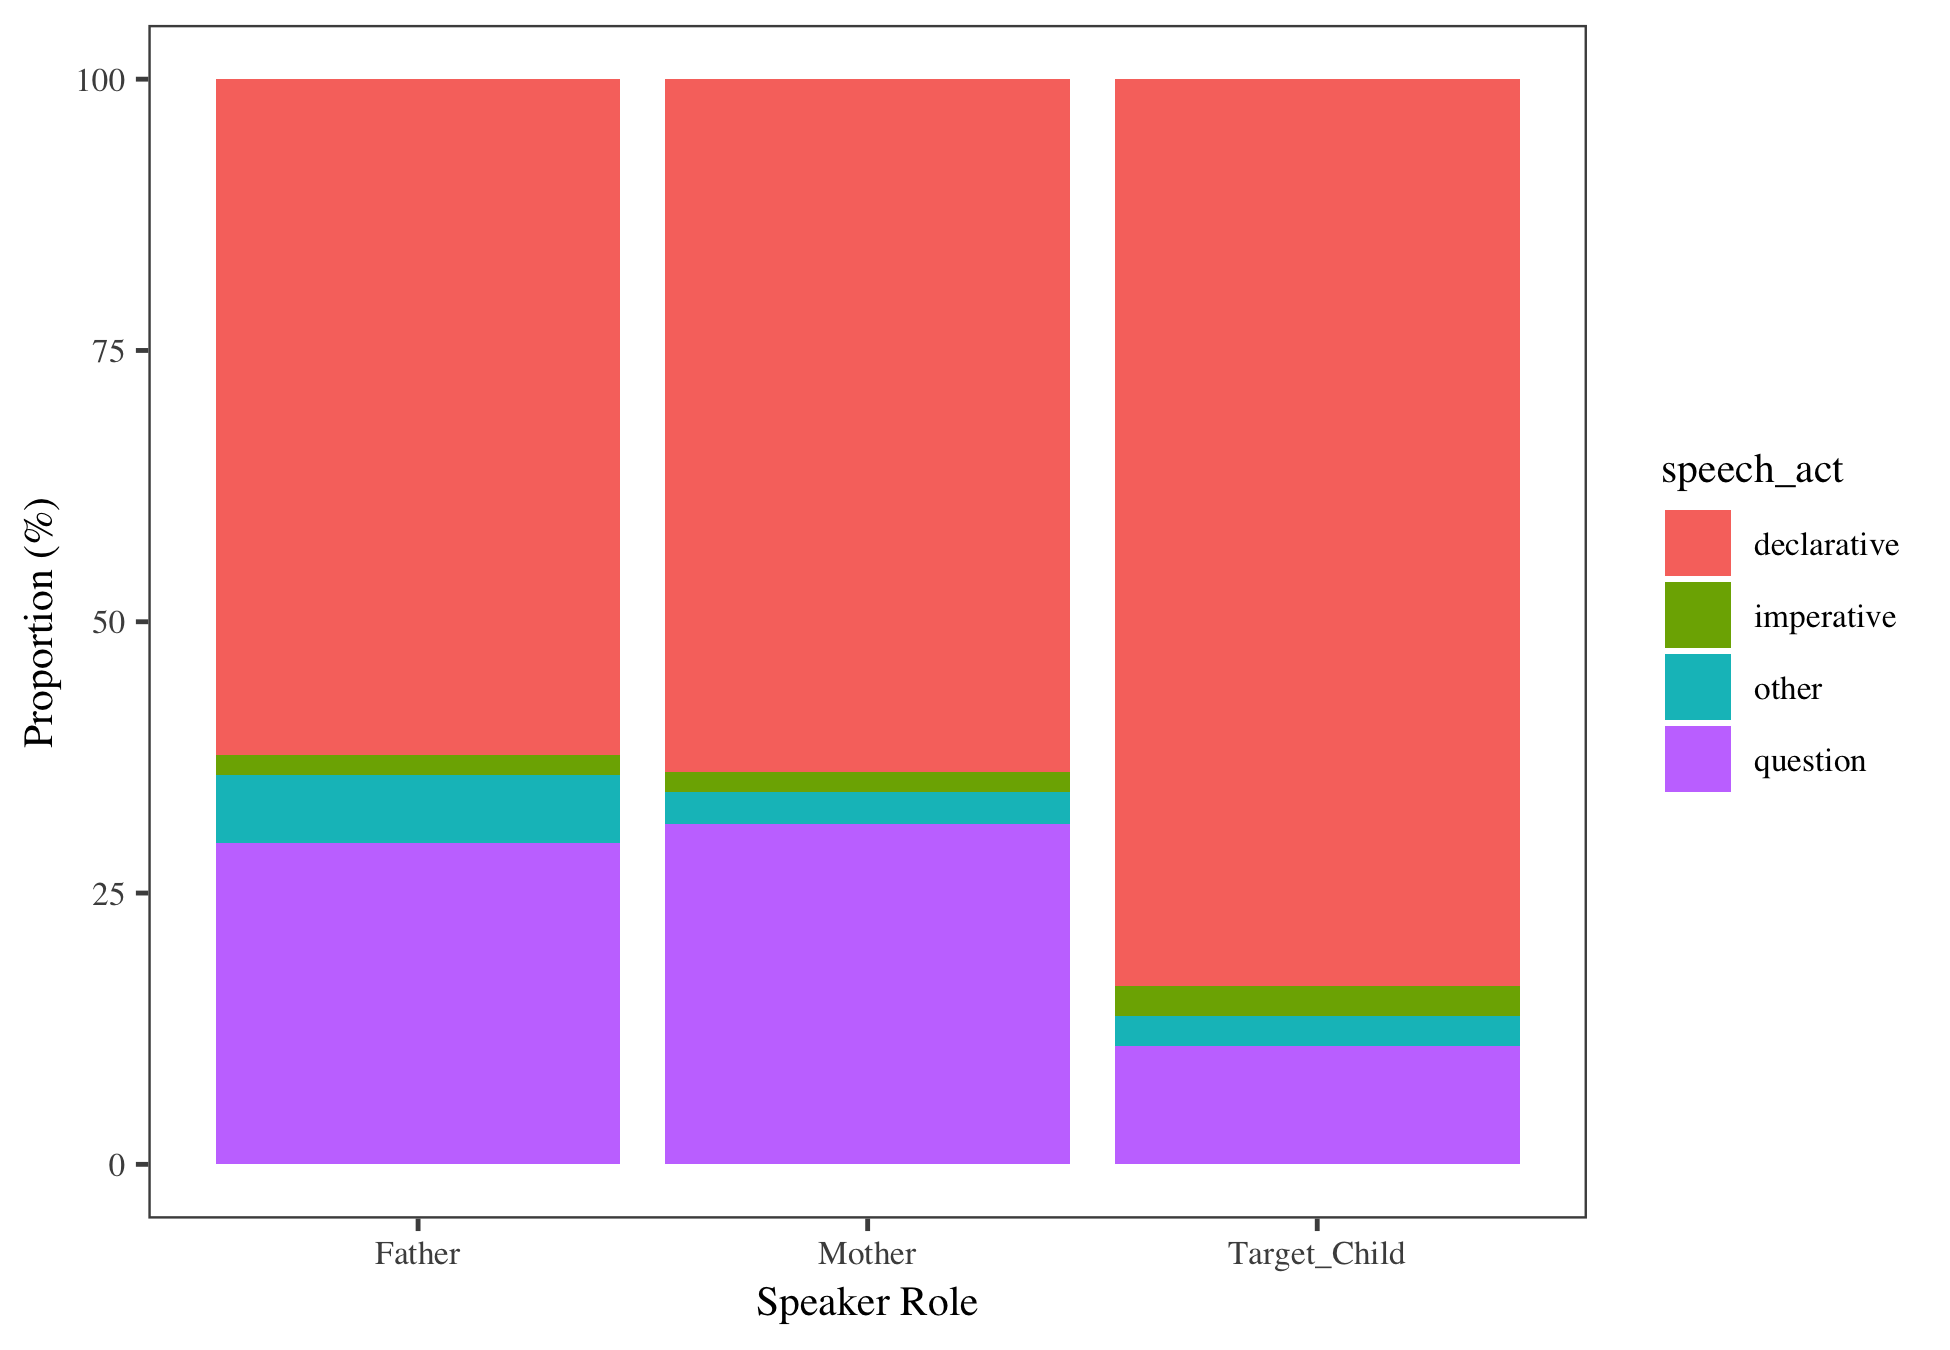
\includegraphics{figs/totalUtteranceTypePlot-1} 

}

\caption{The proportion of declaratives and questions in children's and parents' utterances.}\label{fig:totalUtteranceTypePlot}
\end{figure}

Figure \ref{fig:utteranceTypeByAgePlot} shows the developmental trend of
declaratives and questions between the ages of one and six. Children
start with only producing declaratives and add non-declarative
utterances to their repertoire gradually until they get closer to the
parents' rate around the age six. They also start with very few
questions and increase the number of questions they ask gradually. It is
important to note that the rates of declaratives and questions in
children's speech do not reach the adult rate. These two figures show
that parent-child interactions are asymmetric. Parents ask more
questions and children produce more declaratives. This asymmetry also
interacts with age: the speech of younger children has a higher
proportion of declaratives than older children.

\begin{figure}
\centering
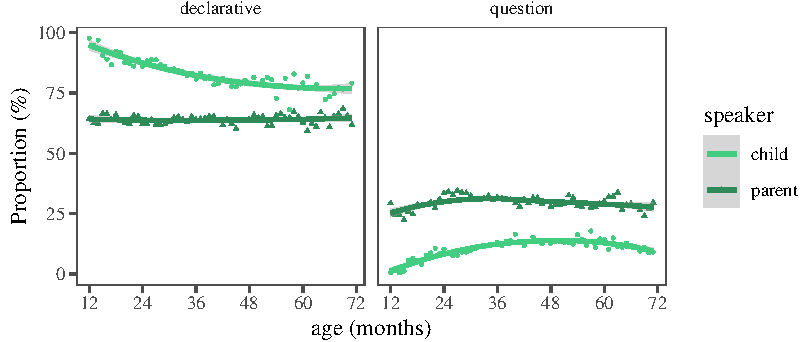
\includegraphics{figs/utteranceTypeByAgePlot-1.pdf}
\caption{\label{fig:utteranceTypeByAgePlot}Proportion of declaratives to
questions in parent-child interactions by age.}
\end{figure}

The frequency of function words such as \emph{and} and \emph{or} may be
affected by such conversational asymmetries if they are more likely to
appear in some utterance types than others. Figure
\ref{fig:CnctPropbySpeechAct} shows the proportion of
\emph{and}\enquote{s and \emph{or}'s that appear in different utterance
types in parents} and children's speech. In parents' speech, \emph{and}
appears more often in declaratives (around 60\% in declaratives and 20\%
in questions). On the other hand, \emph{or} appears more often in
questions than declaratives, although this difference is small in
mothers. In children's speech, both \emph{and} and \emph{or} appear most
often in declaratives. However, children have a higher proportion of
\emph{or} in questions than \emph{and} in questions.

The differences in the distribution of utterance types can affect our
interpretation of the corpus data on function words such as \emph{and}
and \emph{or} in three ways. First, since the collection contains more
declaratives than questions, it may reflect the frequency and diversity
of function words like \emph{and} that appear in declaratives better.
Second, since children produce more declaratives and fewer questions
than parents, we may underestimate children's knowledge of function
words like \emph{or} that are frequent in questions. Third, given that
the percentage of questions in the speech of children increases as they
get older, function words like \emph{or} that are more likely to appear
in questions may appear infrequent in the early stages and more frequent
in the later stages of children's development. In other words, function
words like \emph{or} that are common in questions may show a seeming
delay in production which is possibly due to the development of
questions in children's speech. Therefore, in studying children's
productions of function words, it is important to look at their relative
frequencies in different utterance types as well as the overall trends.
This is the approach I pursue in the next section.

\begin{figure}[tb]

{\centering 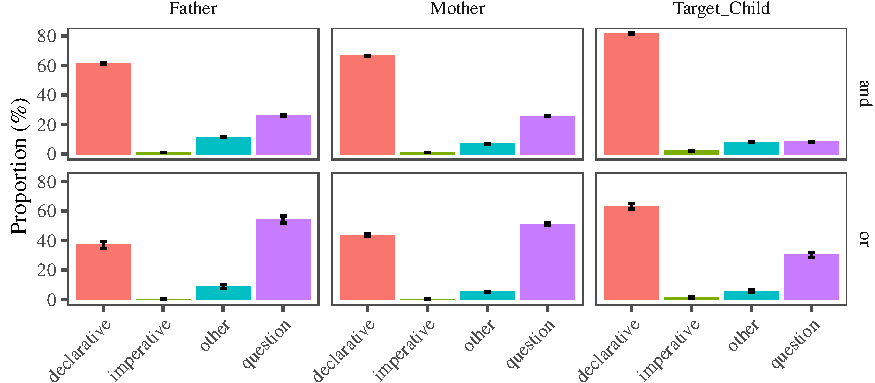
\includegraphics{figs/CnctPropbySpeechAct-1} 

}

\caption{The proportion of \textit{and} and \textit{or} in different utterance types in the speech of parents and children.}\label{fig:CnctPropbySpeechAct}
\end{figure}

\subsubsection{Results}\label{study1results}

First, I consider the overall distribution of \emph{and} and \emph{or}
in the corpora and then look closer at their distributions in different
utterance types. Figure \ref{fig:freqTableBySpeakerPlot} shows the
frequency of \emph{and} and \emph{or} relative to the total number of
words produced by each speaker (i.e.~fathers, mothers, and children).
The y-axes show relative frequency per thousand words. It is also
important to note that the y-axes show different ranges of values for
\emph{and} vs. \emph{or}. This is due to the large difference between
the relative frequencies of these connectives. Overall, \emph{and}
occurs around 15 times per thousand words but \emph{or} only occurs 3
times per 2000 words in the speech of parents and around 1 time every
2000 words in the speech of children. Comparing the relative frequency
of the connectives in parents' and children's speech, we can see that
overall, children and parents produce similar rates of \emph{and} in
their interactions. However, children produce fewer \emph{or}'s than
their parents.

\begin{figure}[tb]

{\centering 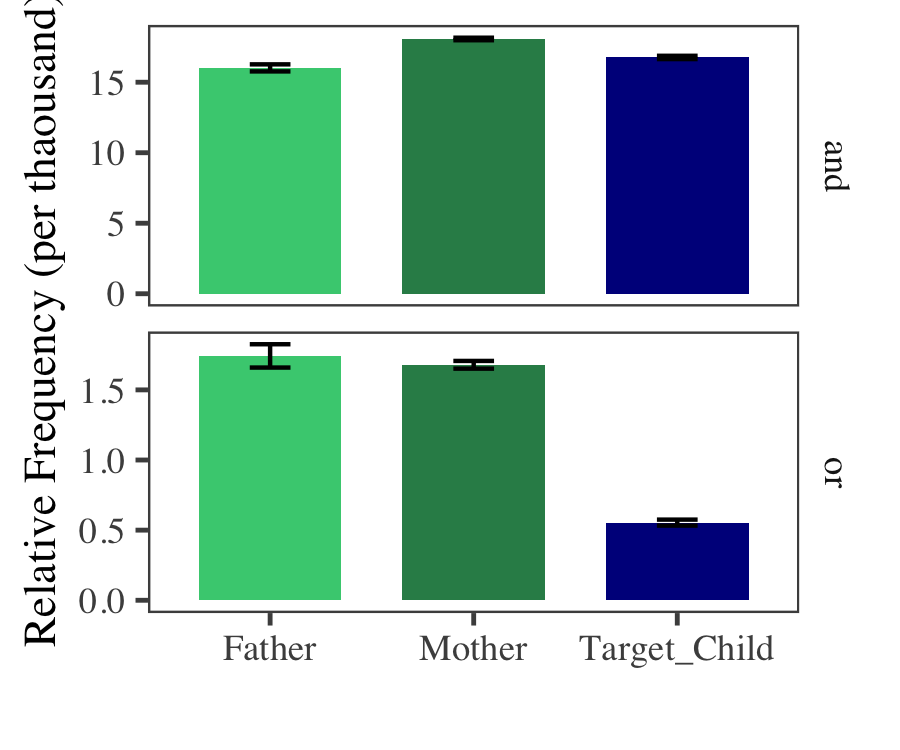
\includegraphics{figs/freqTableBySpeakerPlot-1} 

}

\caption{The relative frequency of \textit{and/or} in the speech of fathers, mothers, and children. 95\% binomial proportion confidence intervals calculated using Agresti-Coull's approximate method.}\label{fig:freqTableBySpeakerPlot}
\end{figure}

Next we look at the relative frequencies of \emph{and} and \emph{or} in
parents and children's speech during the course of children's
development. Figure \ref{fig:agePlot} shows the relative frequencies of
\emph{and} and \emph{or} in parents' and children's speech between 12
and 72 months (1-6 years). Production of \emph{and} in parents' speech
seems to be relatively stable and somewhere between 10 to 20
\emph{and}\enquote{s per thousand words over the course of children's
development. For children, they start producing \emph{and} between 12
and 24 months, and show a sharp increase in their production until they
reach the parent level between 30 to 36 months of age. Children stay
close to the parents} production level between 36 and 72 months,
possibly surpassing them a bit at 60 months -- although as stated in the
previous section, we should be cautious about patterns after 60 months
due to the small amount of data in this period. For \emph{or}, parents
produce between 1 to 2 \emph{or}'s every thousand words and mothers show
a slight increase in their productions between 12 to 36 months. Children
start producing \emph{or} between 18 to 30 months of age. They show a
steady increase in their productions of \emph{or} until they get close
to 1 \emph{or} per thousand words at 48 months (4 years) and stay at
that level until 72 months (6 years).

Children's productions of \emph{and} and \emph{or} show two main
differences. First, the onset of \emph{or} production is later than that
of \emph{and}. Children start producing \emph{and} around 1 to 1.5 years
old while \emph{or} productions start around 6 months later. Second,
children's \emph{and} production shows a steep rise and reaches the
parent level of production at three-years old. For \emph{or}, however,
the rise in children's production level does not reach the parent level
even though it seems to reach a constant level between the ages of 4 and
6 years.

Not reaching the parent level of \emph{or} production does not
necessarily mean that children's understanding of \emph{or} has not
fully developed yet. It can also be due to the nature of parent-child
interactions. For example, since parents ask more questions than
children and \emph{or} appears frequently in questions, parents may have
a higher frequency of \emph{or}. There are two ways of controlling for
this possibility. One is to research children's speech to peers.
Unfortunately such a large database of children's speech to peers is not
currently available for analysis. Alternatively, we can look at the
relative frequencies and developmental trends within utterance types
such as declaratives and questions to see if we spot different
developmental trends. This is what I pursue next. \newline

\begin{figure}[tb]

{\centering 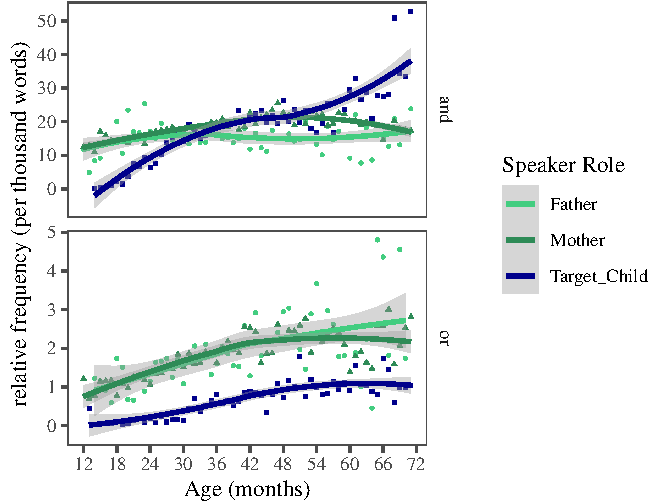
\includegraphics{figs/agePlot-1} 

}

\caption{The monthly relative frequency of \textit{and/or} in parents and children's speech between 12 and 72 months (1-6 years).}\label{fig:agePlot}
\end{figure}

Figure \ref{fig:freqTablebySpeechAct} shows the relative frequency of
\emph{and} and \emph{or} in declaratives, questions, and imperatives.
\emph{And} has the highest relative frequency in declaratives while
\emph{or} has the highest relative frequency in questions. Figure
\ref{fig:ageSpeechActPlot} shows the developmental trends of the
relative frequencies of \emph{and} and \emph{or} in questions and
declaratives. Comparing \emph{and} in declaratives and questions, we see
that the onset of \emph{and} productions are slightly delayed for
questions but in both declaratives and questions, \emph{and} productions
reach the parent level around 36 months (3 years). For \emph{or}, we see
a similar delay in questions compared to declaratives. Children start
producing \emph{or} in declaratives at around 18 months but they start
producing \emph{or} in questions at 24 months. Production of \emph{or}
increases in both declaratives and questions until it seems to reach a
constant rate in declaratives between 48 and 72 months. The relative
frequency of \emph{or} in questions continues to rise until 60 months.
Comparing figures \ref{fig:agePlot} and \ref{fig:ageSpeechActPlot}, we
see that children are closer to the adult rate of production in
declaratives than questions. The large difference between parents and
children's production of \emph{or} in figure \ref{fig:agePlot} may
partly be due to the development of \emph{or} in questions. Overall the
results show that children have a substantial increase in their
productions of \emph{and} and \emph{or} between 1.5 to 4 years of age.
Therefore, it is reasonable to expect that early mappings for the
meaning and usage of these words develop in this age range.

\begin{figure}[tb]

{\centering 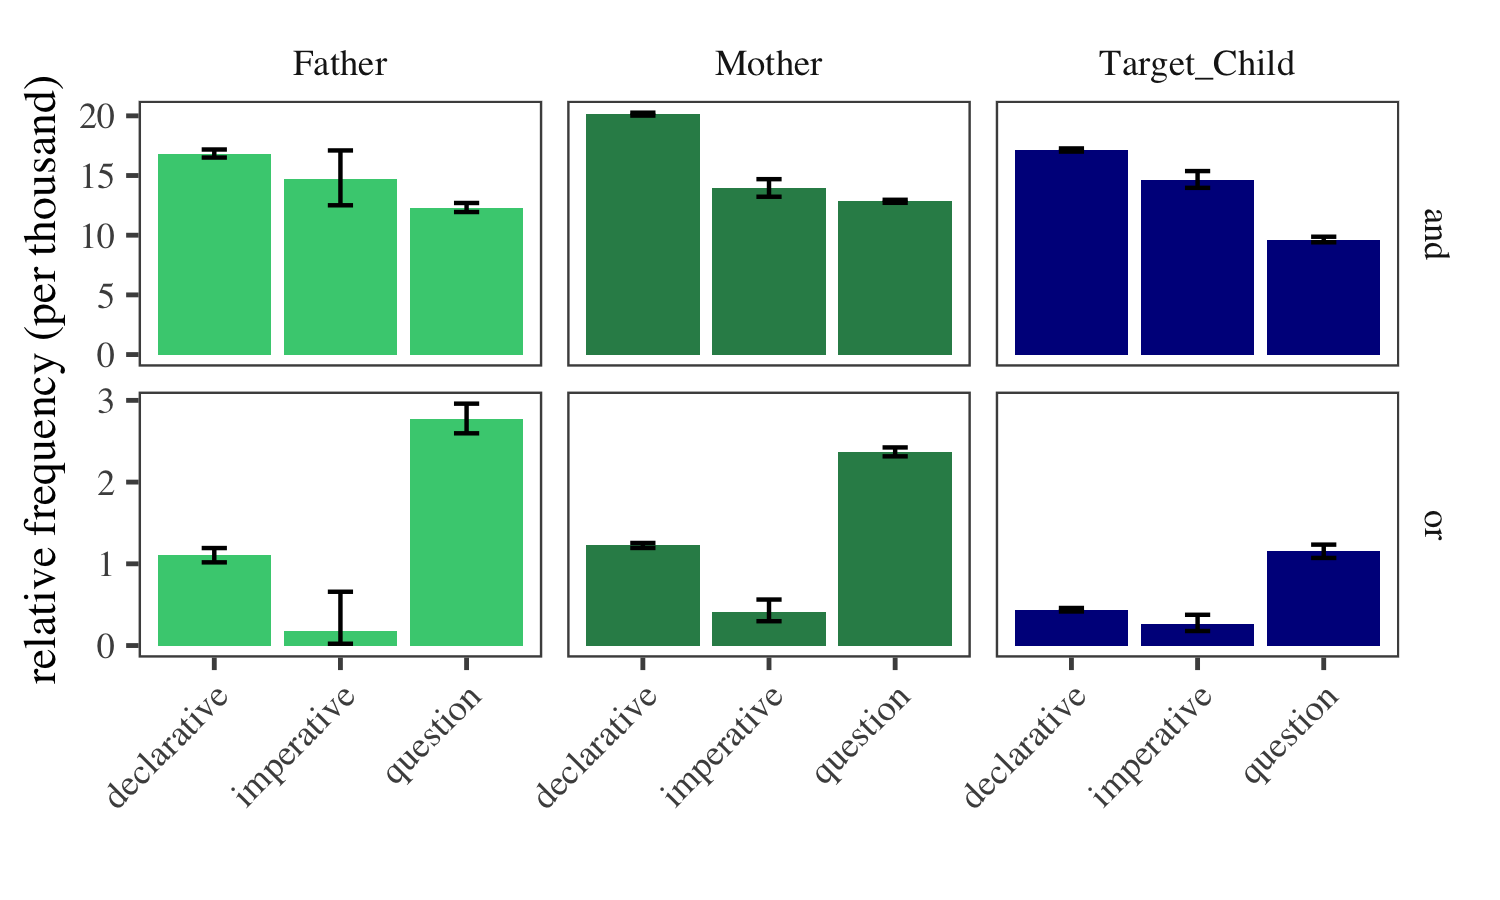
\includegraphics{figs/freqTablebySpeechAct-1} 

}

\caption{Relative frequency of \textit{and/or} in declaratives, imperatives, and interrogatives for parents and children }\label{fig:freqTablebySpeechAct}
\end{figure}

\begin{figure}[tb]

{\centering 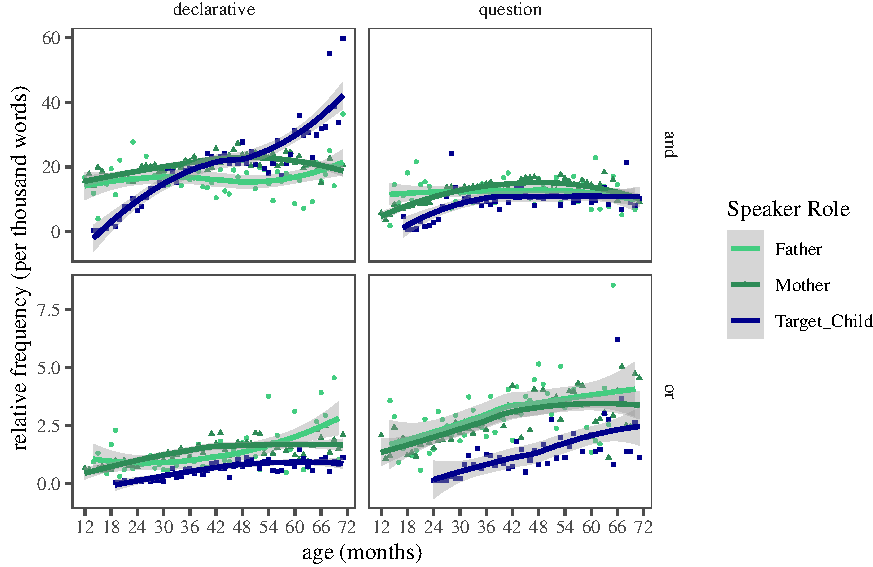
\includegraphics{figs/ageSpeechActPlot-1} 

}

\caption{Relative frequency of \textit{and/or} in declaratives and questions for parents and childern between the child-age of 12 and 72 months (1-6 years).}\label{fig:ageSpeechActPlot}
\end{figure}

\subsubsection{Discussion}\label{study1discussion}

The goal of this study was to explore the frequency of \emph{and} and
\emph{or} in parents and children's speech. The study found three
differences. First, it found a difference between the overall frequency
of \emph{and} and \emph{or} in both parents and children. \emph{And} was
about 10 times more frequent than \emph{or} in the speech of parents and
30 times more likely in the speech of children. Second, the study found
a difference between parents' and children's productions of \emph{or}.
Relative to the total number of words spoken by parents and children
between the ages of 1 and 6 years, both children and parents produce on
average 15 \emph{and}\enquote{s every 1000 words. Therefore, children
match parents} rate of \emph{and} production overall. This is not the
case for \emph{or} as parents produce 3 \emph{or}\enquote{s every 2000
words and children only 1 every 2000 words. Third, the study found a
developmental difference between \emph{and} and \emph{or} as well. The
study found that the onset of production is earlier for \emph{and} than
\emph{or}. In the monthly relative frequencies of \emph{and} and
\emph{or} in the speech of parents and children, the study also found
that children reach the parents} level of production for \emph{and} at
age 3 while \emph{or} does not reach the parents' level even at age 6.

What causes these production differences? The first difference -- that
\emph{and} is far more frequent than \emph{or} -- is not surprising or
limited to child-directed speech. \emph{And} is useful in a large set of
contexts from conjoining elements of a sentence to connecting discourse
elements or even holding the floor and delaying a conversational turn.
In comparison, \emph{or} seems to have a more limited usage. The second
and the third differences -- namely that children produce fewer
\emph{or}\enquote{s than parents, and that they produce \emph{and} and
reach their parents rate earlier than \emph{or} -- could be due to three
factors. First, production of \emph{and} develops and reaches the
parents} rate earlier possibly because it is much more frequent than
\emph{or} in children's input. Previous research suggests that within
the same syntactic category, words with higher frequency in
child-directed speech are acquired earlier (Goodman, Dale, \& Li, 2008).
The conjunction word \emph{and} is at least 10 times more likely than
\emph{or} so earlier acquisition of \emph{and} is consistent with the
effect of frequency on age of acquisition. Second, research on concept
attainment has suggested that the concept of conjunction is easier to
conjure and possibly acquire than the concept of disjunction. In
experiments that participants are asked to detect a pattern in the
classification of cards, participants can detect a conjunctive
classification pattern faster than a disjunctive one (Neisser \& Weene,
1962). Therefore, it is possible that children learn the meaning of
\emph{and} faster and start to produce it earlier but they need more
time to figure out the meaning and usage of \emph{or}.

A third possibility is that the developmental difference between
\emph{and} and \emph{or} is mainly due to the asymmetric nature of
parent-child interactions and the utterance types that each role in this
interaction requires. For example, this study found that parents ask
more questions of children than children do of parents. It also found
that \emph{or} is much more frequent in questions than \emph{and} is.
Therefore, parent-child interaction provides more opportunities for
parents to use \emph{or} than children. In the next study we will
discuss several constructions and communicative functions that are also
more appropriate for the role of parents. For example, \emph{or} is
often used to ask what someone else wants like \enquote{do you want
apple juice or orange juice?} or for asking someone to clarify what they
said such as \enquote{did you mean ball or bowl?}. Both of these
constructions are more likely to be produced by a parent than a child.
\emph{Or} is also used to introduce examples or provide definitions such
as \enquote{an animal, like a rabbit, or a lion, or a sheep}. It is very
unlikely that children would use such constructions to define terms for
parents! Furthermore, such constructions also reveal their own
developmental trends. For example, the study found that children start
by almost entirely producing declaratives and increase their questions
until at age 4 to 6, about 10\% of their utterances are questions.
Therefore, children's ability to produce \emph{or} in a question is
subject to the development of questions themselves. More generally, the
developmental difference between \emph{and} and \emph{or} may also be
due to a difference in the development of other factors that production
of \emph{and} and \emph{or} rely on, such as the development of
constructions with specific communicative functions like unconditionals
(Whether X or Y, discussed in Chapter \ref{sempragLit}). In future
research, it will be important to establish the extent to which each of
these potential causes -- frequency, conceptual complexity, and the
development of other factors such as utterance type or constructions
with specific communicative functions -- contribute to the developmental
differences in the production of conjunction and disjunction.

\section{Study 3: Learning to interpret a
disjunction}\label{study-3-learning-to-interpret-a-disjunction}

\section{Conclusion}\label{conclusion}

\newpage

\section{References}\label{references}

\section{Appendix}\label{appendix}

\subsection{Inter-annotator agreement}\label{inter-annotator-agreement}

\setlength{\parindent}{-0.5in} \setlength{\leftskip}{0.5in}

\hypertarget{refs}{}
\hypertarget{ref-goodman2008does}{}
Goodman, J. C., Dale, P. S., \& Li, P. (2008). Does frequency count?
Parental input and the acquisition of vocabulary. \emph{Journal of Child
Language}, \emph{35}(3), 515--531.

\hypertarget{ref-macwhinney2000childes}{}
MacWhinney, B. (2000). \emph{The CHILDES project: The database} (Vol.
2). Mahwah, NJ: Erlbaum.

\hypertarget{ref-morris2008logically}{}
Morris, B. J. (2008). Logically speaking: Evidence for item-based
acquisition of the connectives ``and'' and ``or''. \emph{Journal of
Cognition and Development}, \emph{9}(1), 67--88.

\hypertarget{ref-neisser1962hierarchies}{}
Neisser, U., \& Weene, P. (1962). Hierarchies in concept attainment.
\emph{Journal of Experimental Psychology}, \emph{64}(6), 640.

\hypertarget{ref-sanchez2018childes}{}
Sanchez, A., Meylan, S., Braginsky, M., MacDonald, K., Yurovsky, D., \&
Frank, M. C. (2018). Childes-db: A flexible and reproducible interface
to the child language data exchange system. PsyArXiv. Retrieved from
\url{psyarxiv.com/93mwx}






\end{document}
